\documentclass[11pt]{article}
\usepackage[margin=0.4in, landscape]{geometry} % Minimized margins to gain maximum whitespace
\usepackage{tikz}
\usetikzlibrary{automata, positioning, arrows.meta, shapes.geometric}

\begin{document}

\thispagestyle{empty} % Eliminates header/footer placeholders completely
\noindent

\begin{center}
% Title made inline and small to prevent triggering page breaks
\textsf{\textbf{\large Ray Tracing State Machine Architecture}}
\end{center}
\vspace{-0.2cm}

\begin{center}
% Scaling dynamically based on height (!) to guarantee it clears vertical page constraints
\resizebox{!}{0.78\textheight}{%
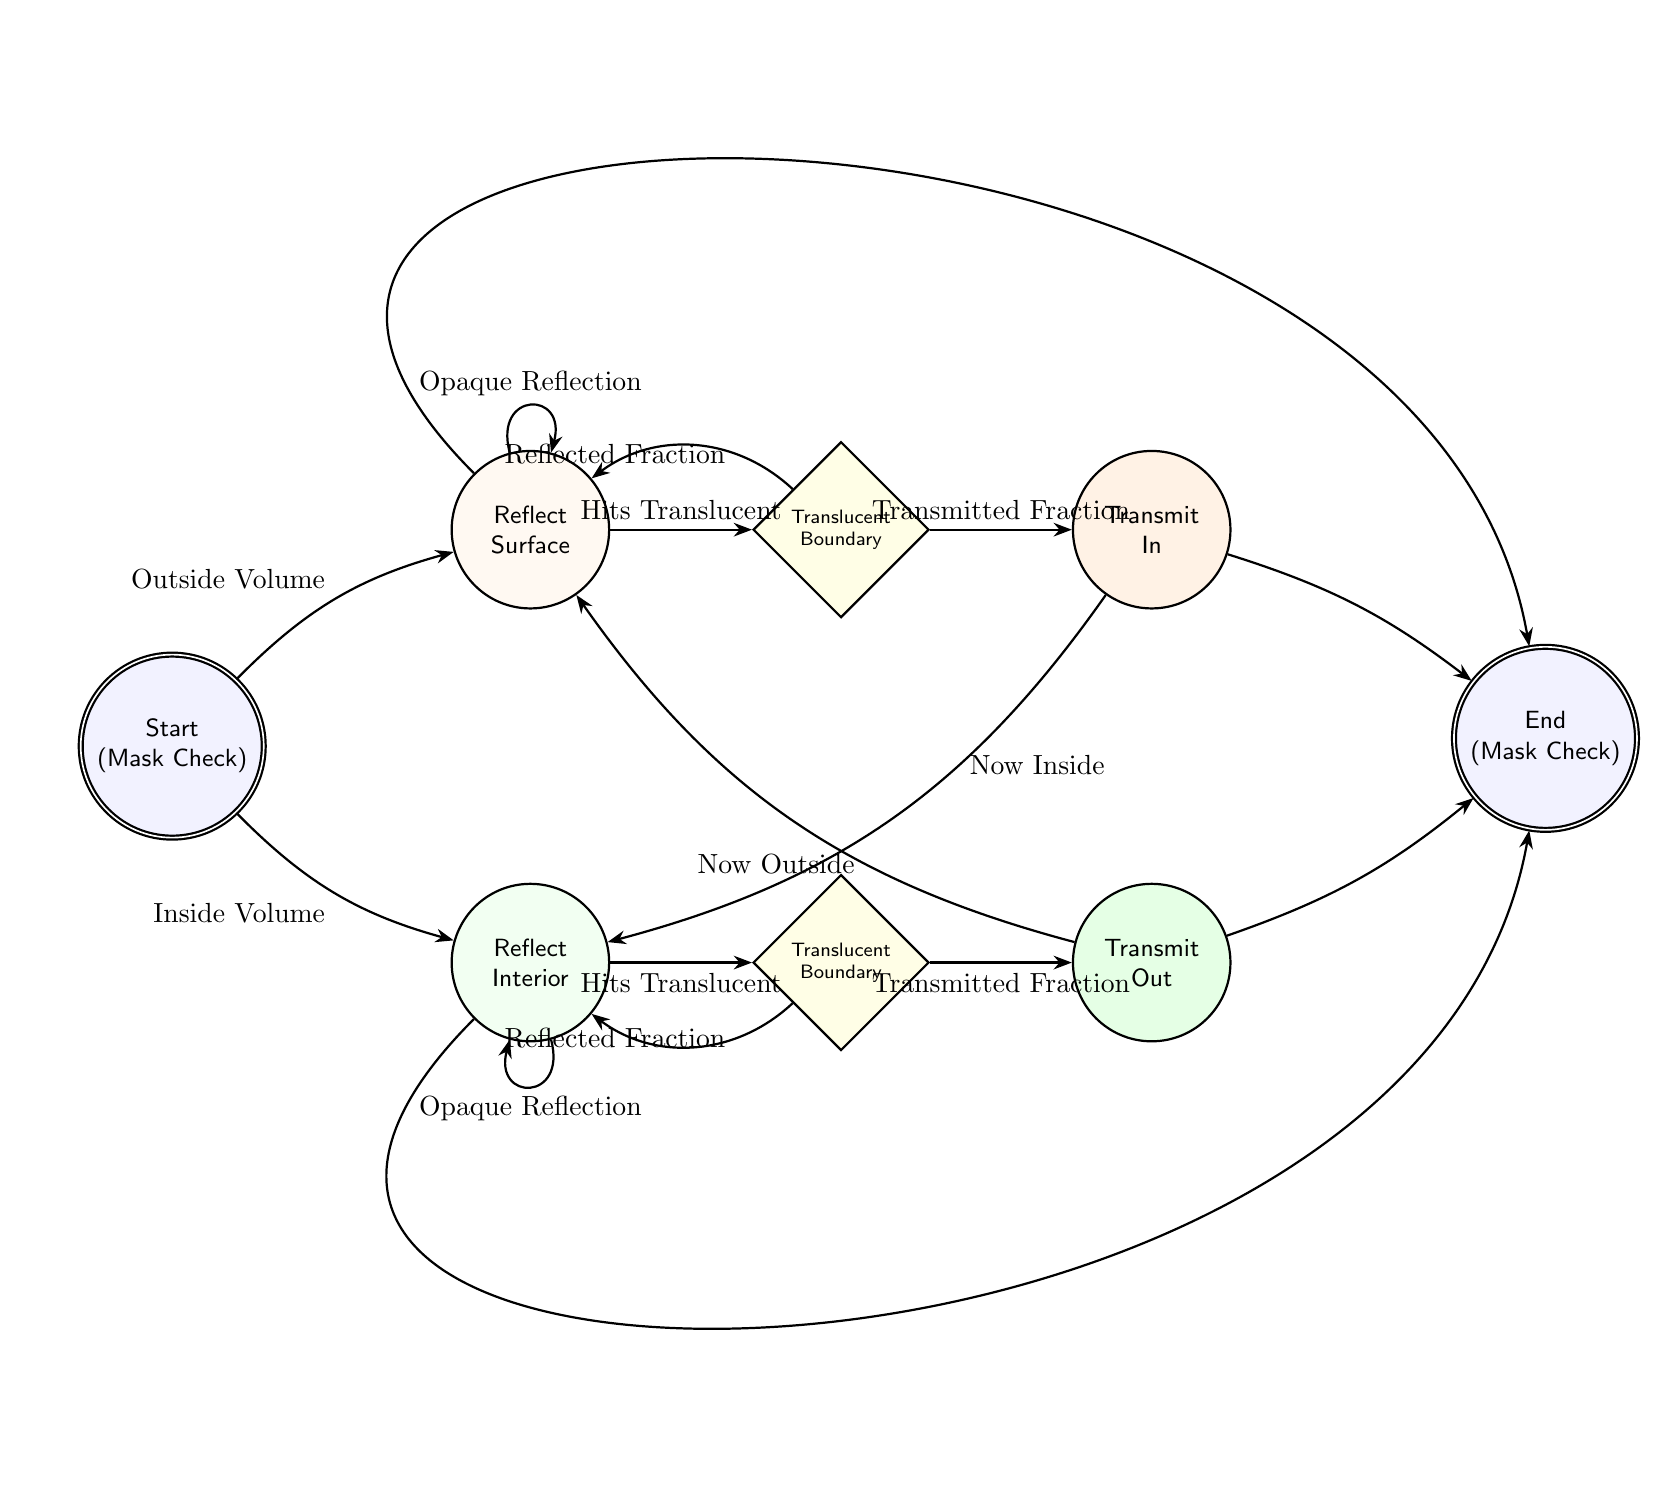
\begin{tikzpicture}[
    >=Stealth,
    node distance=2.2cm and 3.5cm, % Slightly tightened to preserve text scaling ratio
    every state/.style={thick, fill=blue!5, minimum size=2.0cm, align=center, font=\small\sffamily},
    split/.style={diamond, draw, thick, fill=yellow!10, minimum size=1.2cm, font=\scriptsize\sffamily, align=center},
    auto
]

    % --- Column 1: Unified Entry State (Far Left) ---
    \node[state, double] (startmask) {Start\\(Mask Check)};
    
    % --- Column 2: Reflection/Interaction Domains ---
    \node[state, above right=1.2cm and 3.0cm of startmask, fill=orange!5] (refsurf) {Reflect\\Surface};
    \node[state, below right=1.2cm and 3.0cm of startmask, fill=green!5] (refint) {Reflect\\Interior};
    
    % --- Column 3: Translucent Interface Bifurcations ---
    \node[split, right=1.8cm of refsurf] (extsplit) {Translucent\\Boundary};
    \node[split, right=1.8cm of refint] (intsplit) {Translucent\\Boundary};

    % --- Column 4: Transmission Vectors ---
    \node[state, right=1.8cm of extsplit, fill=orange!10] (transin) {Transmit\\In};
    \node[state, right=1.8cm of intsplit, fill=green!10] (transout) {Transmit\\Out};

    % --- Column 5: Unified Accepting Exit Node (Far Right) ---
    \node[state, accepting, right=2.8cm of transin, yshift=-2.65cm] (endmask) {End\\(Mask Check)};

    % --- Explicitly Routed Connections ---
    \path[->, thick] 
        % Router to Spatial Domains
        (startmask) edge[bend left=15] node[above left] {Outside Volume} (refsurf)
        (startmask) edge[bend right=15] node[below left] {Inside Volume} (refint)
        
        % Pure Opaque Reflection Loops 
        (refsurf) edge[loop above, looseness=4] node[above] {Opaque Reflection} (refsurf)
        (refint) edge[loop below, looseness=4] node[below] {Opaque Reflection} (refint)

        % Interface Transitions
        (refsurf) edge node[above] {Hits Translucent} (extsplit)
        (refint) edge node[below] {Hits Translucent} (intsplit)
        
        % Split Outputs (Bifurcations)
        (extsplit) edge[bend right=40] node[left, pos=0.3] {Reflected Fraction} (refsurf)
        (extsplit) edge node[above] {Transmitted Fraction} (transin)
        
        (intsplit) edge[bend left=40] node[left, pos=0.3] {Reflected Fraction} (refint)
        (intsplit) edge node[below] {Transmitted Fraction} (transout)
        
        % Domain Crossings (Post-Transmission Cross-Over Paths)
        (transin) edge[bend left=20] node[right, pos=0.35] {Now Inside} (refint)
        (transout) edge[bend left=20] node[left, pos=0.35] {Now Outside} (refsurf)
        
        % Inner Termination Paths to End Mask
        (transin) edge[bend left=10] (endmask)
        (transout) edge[bend right=10] (endmask);

    % --- Outer-most Perimeter Sinks (Sweeping completely clear of outer loops) ---
    \path[->, thick]
        (refsurf) edge[out=135, in=100, looseness=1.5] (endmask)
        (refint) edge[out=-135, in=-100, looseness=1.5] (endmask);

\end{tikzpicture}%
}
\end{center}

\end{document}
